\begin{figure*}[t!]
\centering
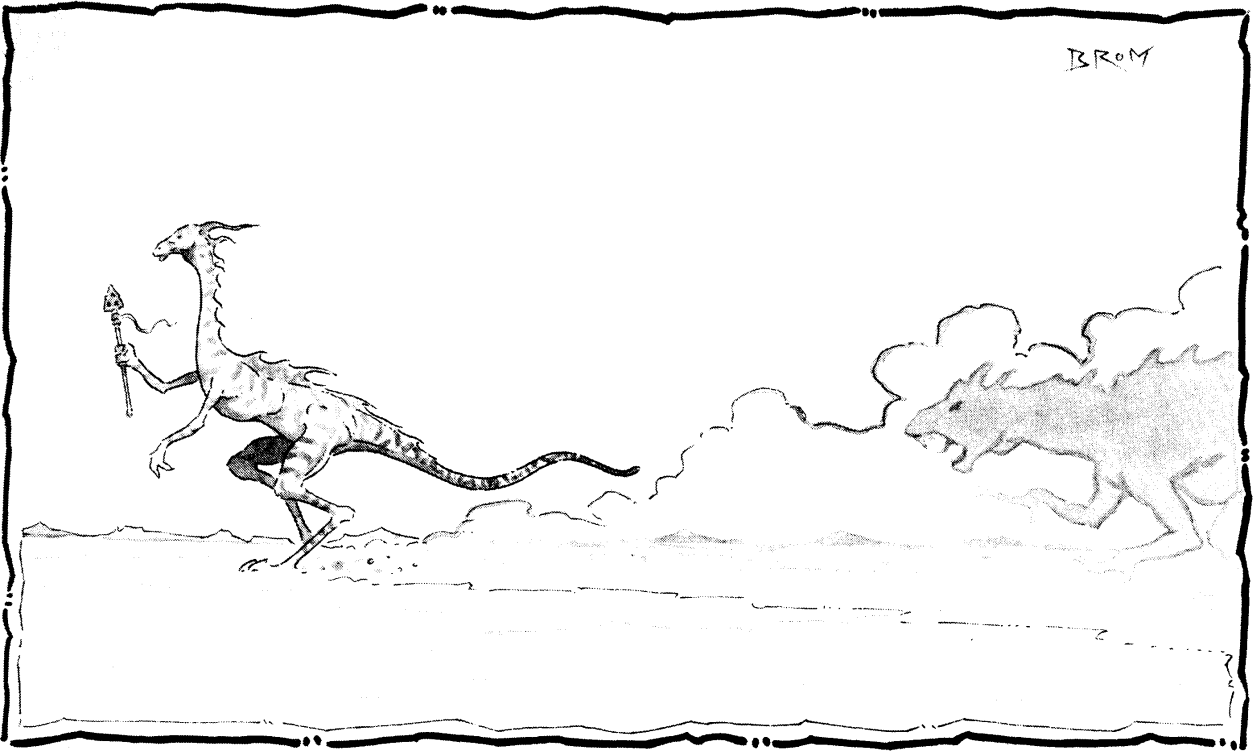
\includegraphics[width=\textwidth]{images/jozhal.png}
\WOTC
\end{figure*}

\subsectionA{Jozhal}
Jozhals are small, lightly built reptilian creatures which may be distantly related to crodlu. They have long, slender legs, lanky arms ending in dexterous hands, and long, flexible tails. The neck of a jozhal is also long and flexible, ending in a narrow-muzzled head with large eyes and many needle-like teeth. The skin is covered in many tiny scales, which are only visible on close examination, and can change color to match with or contrast against the creature's surroundings. Jozhals have precise control over their skin's color, and sometimes use it to create decorative patterns of color resembling tattoos.

\subsubsection{Jozhal Society}
Jozhals are naturally shy and secretive creatures, and do not normally learn the languages of other races. The leader of a family will learn the Common tongue, so that he or she may communicate with outsiders on the rare occasion that interaction is necessary. When around those they do not know, especially other races, jozhals become much more withdrawn and are unwilling to even speak to outsiders unless necessary. They will often travel days out of their way just to avoid encountering non-jozhals, especially elves and humans, whom they consider destructive. If forced to interact with members of another race, jozhals will attempt to make the experience as short as possible. Jozhals do not normally form permanent settlements. Instead, they travel in nomadic family groups, traveling between the fertile areas of the Tablelands and Hinterlands, beyond the Ringing Mountains. These families forage for roots, nuts, and small reptiles and insects. Jozhals always make use of every little bit of anything that they find, to the point of extremes, practicing cannibalism and fashioning the bones of their dead into weapons and tools. The only time a jozhal family will permanently settle in one area is when a member of that family becomes a grove master and takes custody of his guardian lands.

Jozhals are deeply suspicious of all arcane spellcasters. They will tolerate preservers, but will watch them closely for any signs that they may defile, and criticize them harshly if they use magic wantonly or carelessly. Jozhals do not tolerate defilers in any way. A jozhal may even put himself at risk to stop a defiler from damaging the land. The jozhal suspicion of arcane magic does not extend to magical items. Jozhals are fascinated by magical items, which they consider to hold the power of the land, and desire to own as may magical items as they can. Jozhal children are taught from a young age the proper use of magical items, both arcane and divine, so even non-spellcaster jozhals will be able to use most any magical item they come to possess. They go to great lengths to possess magical items, typically following parties of humanoids to determine if they carry any magical items and stealing any they detect.

Jozhal is a language composed of click, pops, and whistles. Do to its unusual nature, many who are not familiar with Jozhal will not even recognize it as a language. The vast majority of jozhals do not keep a written form of their language, and the pyreen alphabet is the only known writing system that can be adapted to writing the jozhal tongue.

\subsubsection{Jozhal Racial Traits}
\begin{itemize*}
    \item $-4$ Strength, +4 Dexterity, $-2$ Constitution, +4 Intelligence, +2 Wisdom.
    \item Aberration: jozhals are not subject to spells or effects that affect humanoids only, such as \spell{charm person} or \spell{dominate person}.
    \item Small: jozhals gain a +1 size bonus to Armor Class, a	+1 size bonus on attack rolls, and a +4 size bonus on \skill{Hide} checks, but they must use smaller weapons than humans use, and their lifting and carrying limits are three-quarters of those of a Medium character.
    \item A jozhal's base land speed is 18 meters.
    \item Racial Hit Dice: A jozhal begins with four levels of aberration, which provide 4d8 Hit Dice, a base attack bonus of +3, and base saving throw bonuses of Fort +1, Ref +1 and Will +4.
    \item Racial Skills: A jozhal's aberration levels give it skill points equal to 7 $\times$ (2 + Int modifier). Its class skills are \skill{Climb}, \skill{Concentration}, \skill{Hide}, \skill{Jump}, \skill{Knowledge} (arcana), \skill{Listen}, and \skill{Use Magic Device}.
    \item A jozhal's aberration levels give it 2 feats.
    \item Weapon Proficiency: A jozhal is proficient with all simple weapons and its natural weaponry.
    \item +4 racial bonus on \skill{Hide} checks. Jozhals can alter their skin coloration and often use this for camouflage purposes.
    \item +4 racial bonus on \skill{Use Magic Device} checks. Jozhals have a natural affinity for magic.
    \item Natural Armor: +4 natural armor bonus to AC.
    \item Natural Weapons: Bite (1d8).
    \item Psionic Powers: A jozhal character manifests psionic powers as a 4th-level psion. If the character takes additional levels of psion, these levels stack with the jozhal's base manifesting ability for powers known, power points per day, and other effects dependent on manifester level. A jozhal character likewise uses the sum of its racial spellcasting levels and class levels to determine the abilities of its psicrystal.
    \item Spells: A jozhal character casts spells as a 4th-level elemental cleric---jozhal are never paraelemental clerics. If the character takes additional levels of cleric, these levels stack with the jozhal's base spellcasting ability for spells per day, and other effects dependent on caster level. A jozhal character likewise uses the sum of its racial spellcasting levels and class levels to determine the abilities of their domain granted powers.
    \item Spell Resistance (Ex): A jozhal has spell resistance equal to 9 + class levels.
    \item Automatic Languages: Jozhal, Common. Bonus Languages: Aarakocra, Dwarven, Elven, Pterran, and Thri-Kreen.
    \item Favored Class: Cleric.
    \item Level Adjustment: +5.
\end{itemize*}
